%plan for this chapter

%the boring way first
%- so far we have discussed constraints on reactions for invisible particles
%-- remember that this is all the LHC can do by itself
%- but within a single model and under certain assumptions (detector stable -> cosmologically stable), LHC results can be used to constrain properties of the parameters of DM
%- and so can DD and ID, although they have the advantage that they can be sure that it's cosmologically stable DM 
%- so let's put them together in this chapter, in the context of specific models, and highlight the complementarity between searches that:
%-- know a lot about the interaction itself
%-- can get to the origin


%Note on this figure: it's on wikimedia before i submitted the nature physics because I planned to reuse it here and told nature physics i wanted it cited but nature physics being the predatory shit paper that it is ignored all my request of creative commons (but they redid it with thinner lines). maybe we reword the caption?
\begin{figure}[!htpb]
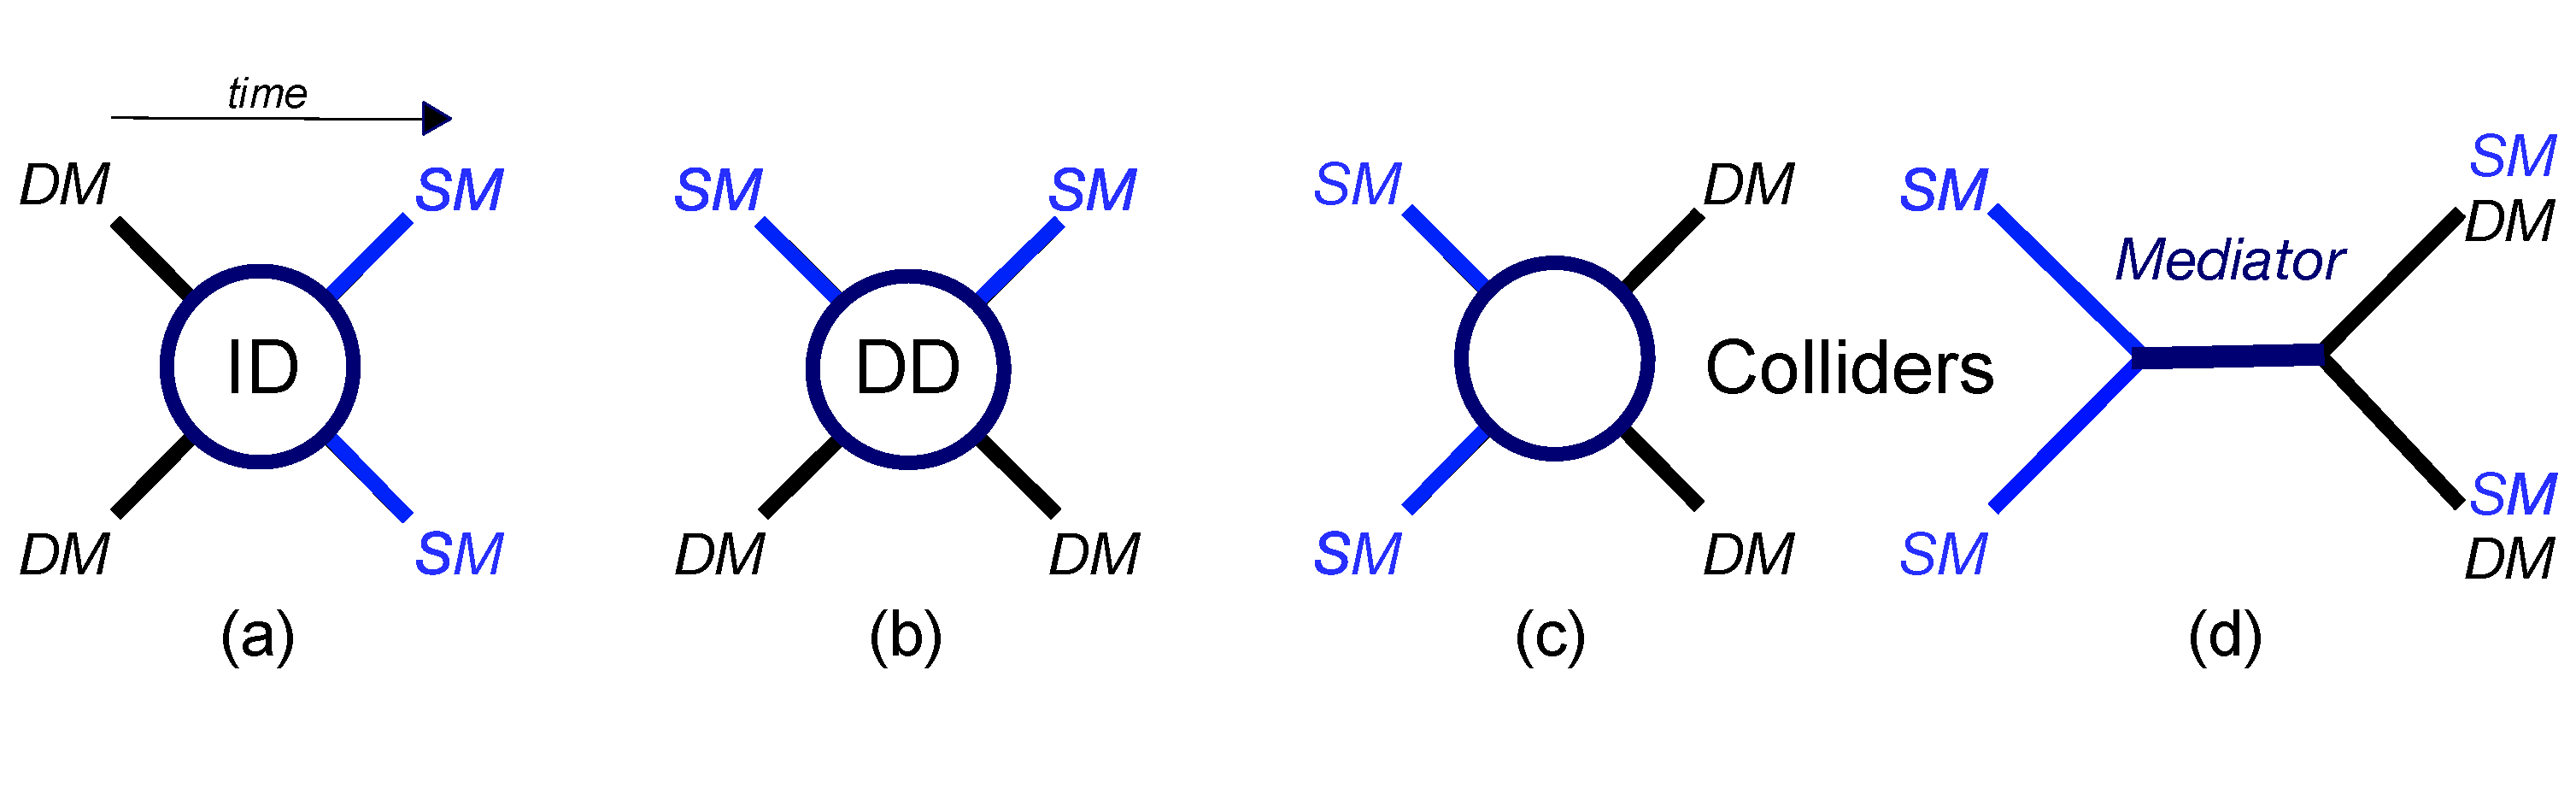
\includegraphics[width=\textwidth]{figures/EFTSimplifiedModels}
\caption{Schematic illustration of Dark Matter interactions and their corresponding experimental detection techniques, with time flowing from left to right. Fig. (a) shows DM annihilation to Standard Model particles, as sought by Indirect Detection (ID) experiments. Fig. (b) shows DM -> SM particle scattering, targeted by Direct Detection (DD) experiments. Fig. (c) shows the production of DM particles from the annihilation of SM particles at colliders. Fig. (d) shows again the pair production of DM at colliders as in (c), but in this case the interaction occurs through a mediator particle between DM and SM particles. From~\cite{monoXfig}, inspired by ~\cite{Bauer:2013ihz}.}
\label{fig:Complementarity}
\end{figure}

%Previous intro was:
%The comparison of results from complementary experiments needs a mechanism to relate the processes
%that will produce a signal in each type of detectors. This ultimately means that any comparison between LHC, DD and ID
%needs a fully specified theoretical benchmark to be predictive and consistent. Since there are a large possible number of options to choose from, 
%it is always important to keep in mind that such comparisons are model-dependent and the choice of benchmark can have severe implications for the conclusions drawn. 

%people just read: we didn't find shit
%make some sort of link with the Z invisible SM surprise
Collider searches are sensitive to a wide variety of reactions for invisible particles, and are particularly suited to probing and characterizing the mediator of the interaction if the mediator is within the reach of the collider energy scale. %bleurgh
So far, no searches have found evidence of excesses over SM processes, constraining the rates of these reactions.
%if constrain, useful 
Within a given model and under well-specified assumptions, these constraints can be related to direct and indirect searches for DM production, since as shown in Fig~\ref{fig:Complementarity} (a-c) SM-DM interactions lead to DM production at collider, scattering at direct detection experiment, and DM annihilation which can lead to signals at indirect detection experiments within standard thermal freeze-out scenario. 
%if discovery, useful
This complementarity of multiple experiments is helpful to elucidate the nature of dark matter in case of a discovery,
by probing the physics processes that complement DM production (e.g. new particles from SUSY cascades, or visible decays of light mediator as in Fig~\ref{fig:Complementarity} (d)), 
and by enabling to connection of a possible collider signal to its cosmological nature. %bleurgh
%what we didn't say: sure, extrapolation requires a model. lhc results are extremely model dependent but that is a feature (learn more about the model)


%what we were asked to do
%We invite you to write a short review on the current searches for dark matter and other invisible particles at the LHC. This review should discuss the important reactions for invisible particle searches, the experimental challenges for observing these reactions, and some of the innovations by ATLAS and CMS that address these challenges. The review should discuss the parameterization of invisible particle cross sections by simplified models, for example, as presented in the recent Dark Matter Forum paper and in the actual practice of ATLAS and CMS. The review should present current results from the LHC experiments. Finally, the review should briefly relate and compare the current LHC results to limits from direct and indirect detection of dark matter. The review should be accessible to students and postdoctoral researchers who would like to enter this area of research.

%what are we going to do (could be cut)
In the following, we outline the strategy adopted by collider experiments to extrapolate their results to cosmological DM DD and ID results, discuss the assumptions made in the relic density calculation, and conclude with relating the constraints on reactions for invisible particles for reactions of DM.
%i really wanted to say the word "consequences of constraints"

\subsection{Comparing LHC constraints from visible and invisible searches with non-collider results}

%%strategy: DMWG
%- why we do things the way we do: colliders compare in mass-mass plane, and then we translate
%- how things look like: collider does not care if SI vs SD
%-- some experiments made us the courtesy of doing a similar thing (cite Pico and CTA
%-- caveats of colliders and caveats of ID/DD: uncertainties

%Simp

%EFT junk
%Tevatron and Run-1 LHC searches mainly used EFTs as the common theoretical ground to compare their constraints on DM across experiments, or full models such as SUSY. EFTs are a good and flexible benchmark model to represent DM interactions in DD and ID experiment, since the momentum transfer of the collision is sufficiently low not to resolve the theory beyond the scale of the interaction and certainly below the electroweak scale. As discussed in Sec.~\ref{sub:EFT}, this is not always the case for high-energy collider experiments. The difference in interaction scales also requires that any operator in the model is evolved from the scale of the LHC collisions to the nuclear scale of DD through renormalization group expansion (RGE)~\cite{DEramo:2014nmf} for full consistency of the results. %is it clear enough that this has to be done for simplified models too? 
%An example of a comparison plot between collider and DD results using EFT operators in the WIMP-nucleon cross-section vs WIMP mass plane\footnote{The formulas to translate LHC limits to this plane can be found in Ref.~\cite{Goodman:2010ku}}, without evolving the operators using RGE but showing the effects of the truncation of the events where the EFT is invalid, is shown for the LHC Run-1 results in Fig.~\ref{fig:SIATLASEFT}. %There isn't enough space to describe the results of the truncation in detail

Comparison of collider and non-collider results have prevalently been performed in the framework of simplified models and of more complete SUSY models, using upper limits on the collider interaction rates of a specific reaction to constrain the parameter space used to constrain interactions and parameters considered in DD and ID. 

Comparison using simplified models presented by LHC experiments have so far privileged vector and axial vector $s-$channel models~\footnote{For reinterpretation of LHC results and their comparisons to DD and ID for scalar and pseudoscalar mediators, also in the context of 2HDM, see e.g.~\cite{Athron:2017kgt,Banerjee:2017wxi,Ipek:2014gua,Bell:2016ekl}}.
LHC experimentalists and theorists within the Dark Matter Working Group have chosen to translate the collider results on visible mediator and invisible DM searches to the nucleon-DM cross-section and ID planes, clearly spelling out parameters and assumptions of the chosen model to convey the model dependence of such comparisons~\cite{Boveia:2016mrp}. 

\begin{figure}[!htpb]
%Can't have both so choose less controversial
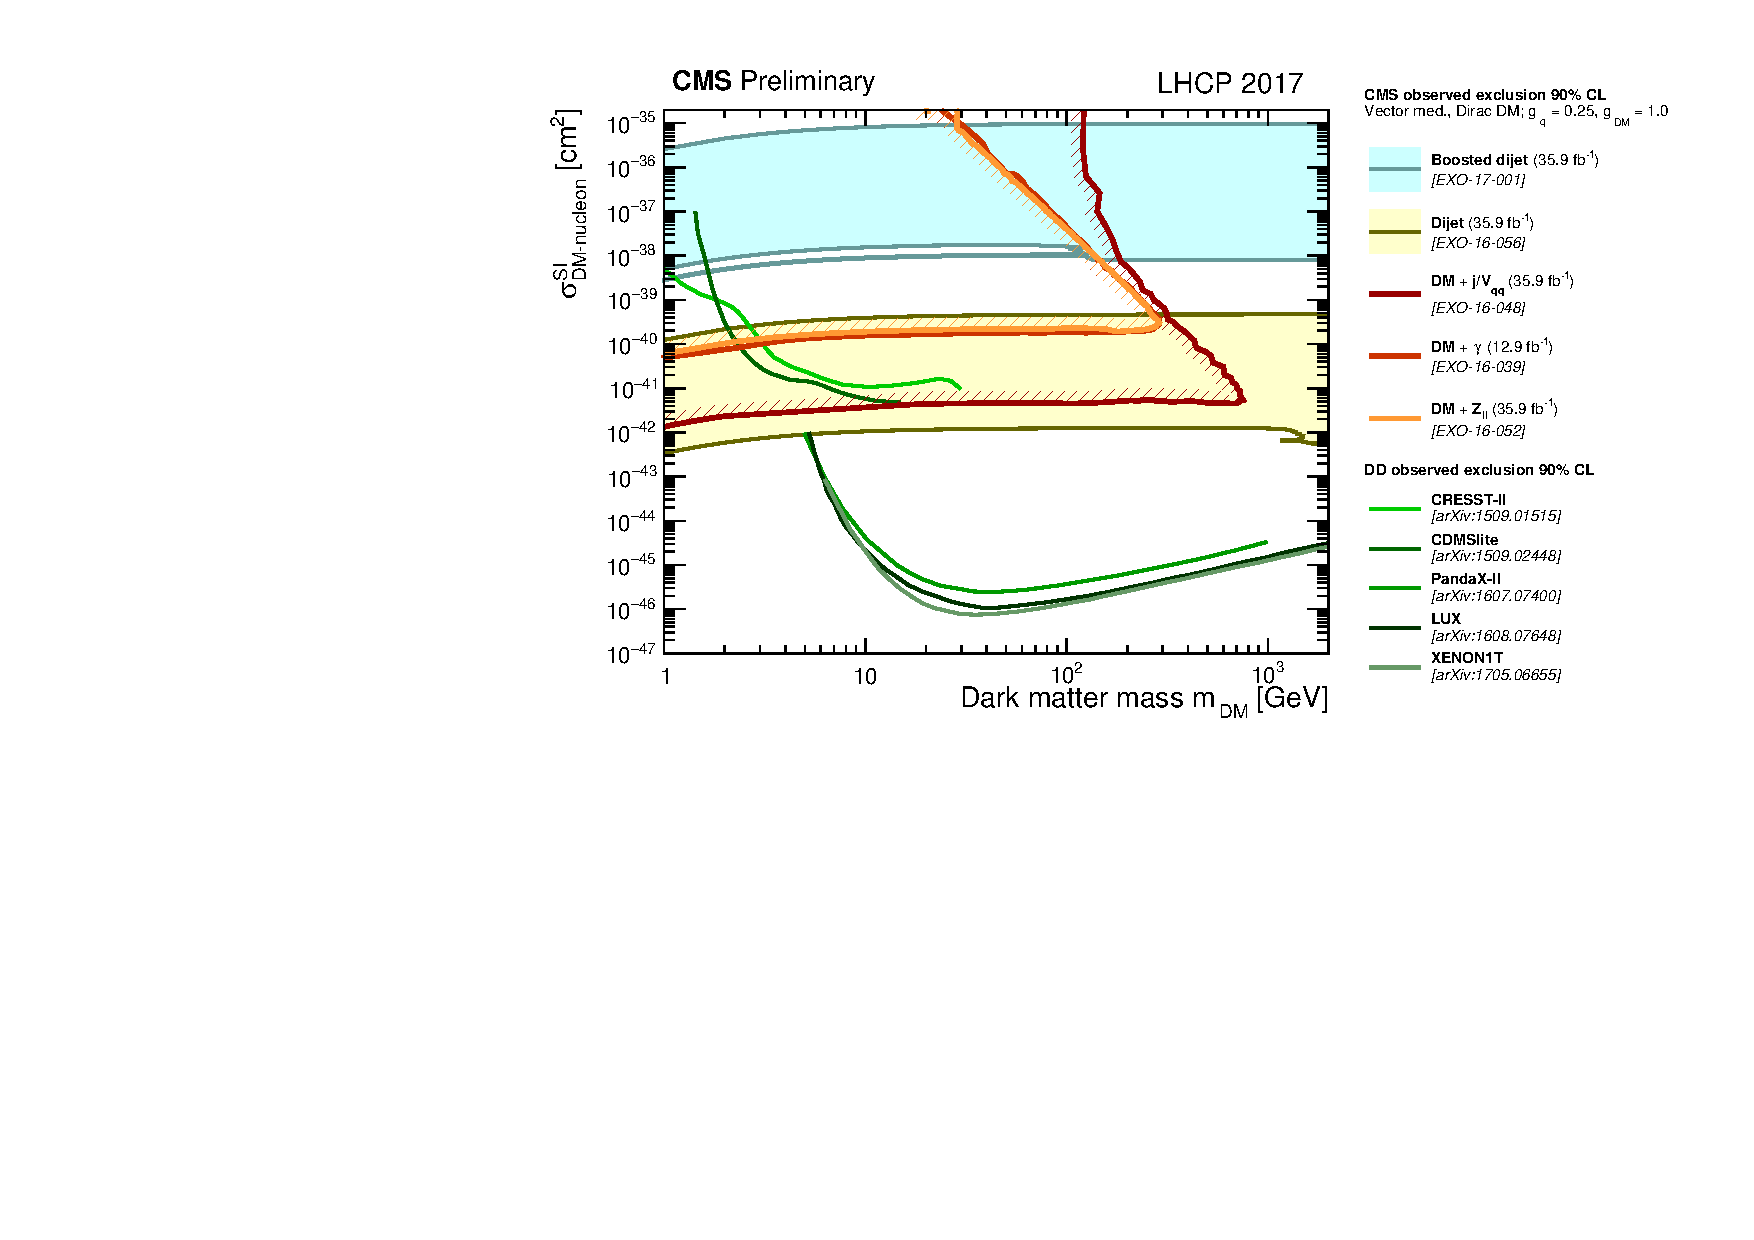
\includegraphics[width=0.9\textwidth]{figures/SI_CMSDD_Summary}
\caption{The 90\% CL constraints from the CMS experiment in the \mdm-spin-independent DM-nucleon plane, for a vector mediator, Dirac DM and couplings \gq = 0.25 and \gdm = 1.0, compared with DD experiments. From~\cite{CMSSummary}.}
%We can update if something else comes out
\label{fig:SICMS}
\end{figure}
%Q: use SD? it will piss off more people but maybe we could make that point as well
%We could cite PDG review on spin-dependent vs spin-independent
%What can be inferred from the plot is that within this class of models and spin assumption %We could have a footnote on SD and SI but no room in text?
%the ideal region for the discovery of DM is that where WIMPs have masses above 10 GeV, as both collider and DD experiments are sensitive and could verify each other's claims. Next-generation DD experiments are expected to lower the minimum sensitivity thresholds in the next decade, see e.g.~\cite{Agnese:2016cpb}. 

An example of such a comparison between the most recent LHC and DD results is shown in Fig.~\ref{fig:SICMS} for a simplified axial vector model. In this kind of comparisons, it should be noted that the exclusion regions obtained from the different collider searches, as well as their relative importance, depend strongly on the benchmark scenario and its couplings. We also note that neither this procedure nor the simplified models used are yet explicitly accounting for effects that may be important for mediators with masses below 100 GeV, such as interference and mixing with SM boson and quarkonia resonances, nor for the evolution of the operators in the model from the LHC collision scale to the nuclear scale of DD~\cite{DEramo:2014nmf}.
Moreover, all experimental results, be it from DD, ID or collider, are affected by experimental and theoretical uncertainties that are not displayed here - we postpone a brief discussion of this topic to Chapter~\cite{sec:05_Future}.

%this is Zurek/Landsberg's point to truncate 
%Proposals exist so that the plots should be truncated for cross-sections corresponding to a minimum mass.  
%Q: mention discussion from Landsberg? Would be nice. 
%https://indico.cern.ch/event/563066/contributions/2306614/attachments/1340042/2017991/DMWG-09-20-16.pdf
%Mention how low can one go in mdm - AB knows better here? 
What can be inferred from the plot is that, within this class of models and interaction Lorentz structure, %We could have a footnote on SD and SI but no room in text?
the ideal region for the discovery of DM is that of intermediate DM masses, as both collider and DD experiments are sensitive and could verify each other's claims. While searches for invisible particles at colliders are sensitive to arbitrarily light DM masses, next-generation DD experiments are expected to lower the minimum sensitivity thresholds for DM-SM recoil in the next decade, see e.g.~\cite{Agnese:2016cpb}. 

%%ID -> LHC
The comparison of collider and ID results using simplified model benchmarks has received further theoretical attention since Ref.~\cite{Boveia:2016mrp}. In traditional comparisons, only one DM annihilation state at a time has been used for the comparison of collider and ID results (e.g. $b\bar{b}$, see for example~\cite{Agrawal:2014una}). The work in~\cite{Carpenter:2016thc} considers multiple final state fermions and interprets ID and LHC results in simplified models with $s-$ and $t-$channel mediators. 
%Could cite this for more consistent w/completion and ID: Jacques:2016dqz, but not sure what it adds, I prefer to talk about Linda's result

Recently, LHC results have also started to be used by DD collaborations to compare the sensitivity to simplified models of DM, see e.g.\cite{PhysRevLett.118.251301,Balazs:2017hxh}. IceCube and other experiments have used constraints from a MSSM scan, see e.g.~\cite{Aartsen:2016zhm}. The pMSSM is also a good framework to highlight the complementarity of LHC, direct and indirect detection experiments, as shown in e.g. Ref,~\cite{Cahill-Rowley:2014twa} and discussed later. %CD: maybe add some quantitative results?

\begin{marginnote}[]
\entry{The LHC Dark Matter Working Group}{provides formulas for the translation of LHC limits to DD and ID in~\cite{Boveia:2016mrp}, as well as calculations of the relic density for a number of coupling choices~\cite{githubDMWG}.} 
\end{marginnote}. 

\subsection{Relic density considerations}

%%relic discussion
%- assumptions in the relic density lines when sticking a simplified model into Micromegas
%-- standard thermal relic, equilibrium then freeze-out
%-- only simplified model is relevant for annihilation
%-- additional ingredients are needed but this is a useful guide

%need to match this with the stuff in the introduction and make sure it does not repeat
The current observed abundance of DM in the universe, derived from fits of the Cosmic Microwave Background measured with the Planck satellite~\cite{Ade:2015xua}, is one of the few %the only? 
available quantitative DM indirect observations. 
As already shown in Fig.~\ref{fig:sensitivityComparison} LHC experiments overlay a line corresponding to  a dark matter density of $\omega_c = 0.12 h^2$ according to the standard thermal history as calculated from programs such as MadDM and MicrOMEGas~\cite{Backovic:2015cra,Barducci:2016pcb}, to illustrate where a given simplified model is sufficient to explain the observed DM abundance. 

Conclusions on whether a model is ruled out by information on relic density alone cannot be drawn for simplified models, as there may be additional physics processes beyond those included in the simplified model that influence the DM abundance.
Moreover, the assumption of a standard thermal history where the current DM density is achieved via freeze-out is only one of the possibilities~\cite{Bernal:2017kxu}. 
%does the reader know what a standard thermal history is?
%how do we treat the assumption of LambdaCDM? way too big a discussion to start here
Nevertheless, the relic density remains a useful guiding principle for DM searches if these assumptions are correct~\cite{Busoni:2014gta,Catena:2017xqq}. 

\subsection{Combined constraints on the parameter space of specific models}

%%results: assorted bag, but at least ordered

%- notes:
%-- colliders are able to arbitrarily go down in DM mass 
%-- mediator masses need care for mixing with Z because precision constraints
%- monoH and monoZ excluded by LEP, DD, ID unless really heavy DM
%- simplified models still have room, and very coupling dependent statement
%- SUSY has megascans but we leave it to others because too much shit (one paragraph)



%%LHC -> DD/ID

%EFT junk
%Tevatron and Run-1 LHC searches mainly used EFTs as the common theoretical ground to compare their constraints on DM across experiments, or full models such as SUSY. EFTs are a good and flexible benchmark model to represent DM interactions in DD and ID experiment, since the momentum transfer of the collision is sufficiently low not to resolve the theory beyond the scale of the interaction and certainly below the electroweak scale. As discussed in Sec.~\ref{sub:EFT}, this is not always the case for high-energy collider experiments. The difference in interaction scales also requires that any operator in the model is evolved from the scale of the LHC collisions to the nuclear scale of DD through renormalization group expansion (RGE)~\cite{DEramo:2014nmf} for full consistency of the results. %is it clear enough that this has to be done for simplified models too? 
%An example of a comparison plot between collider and DD results using EFT operators in the WIMP-nucleon cross-section vs WIMP mass plane\footnote{The formulas to translate LHC limits to this plane can be found in Ref.~\cite{Goodman:2010ku}}, without evolving the operators using RGE but showing the effects of the truncation of the events where the EFT is invalid, is shown for the LHC Run-1 results in Fig.~\ref{fig:SIATLASEFT}. %There isn't enough space to describe the results of the truncation in detail
%What can be inferred from the plot is that within this class of models and spin assumption %We could have a footnote on SD and SI but no room in text?
%the ideal region for the discovery of DM is that where WIMPs have masses above 10 GeV, as both collider and DD experiments are sensitive and could verify each other's claims. Next-generation DD experiments are expected to lower the minimum sensitivity thresholds in the next decade, see e.g.~\cite{Agnese:2016cpb}. 

%\begin{figure}[!htpb]
%%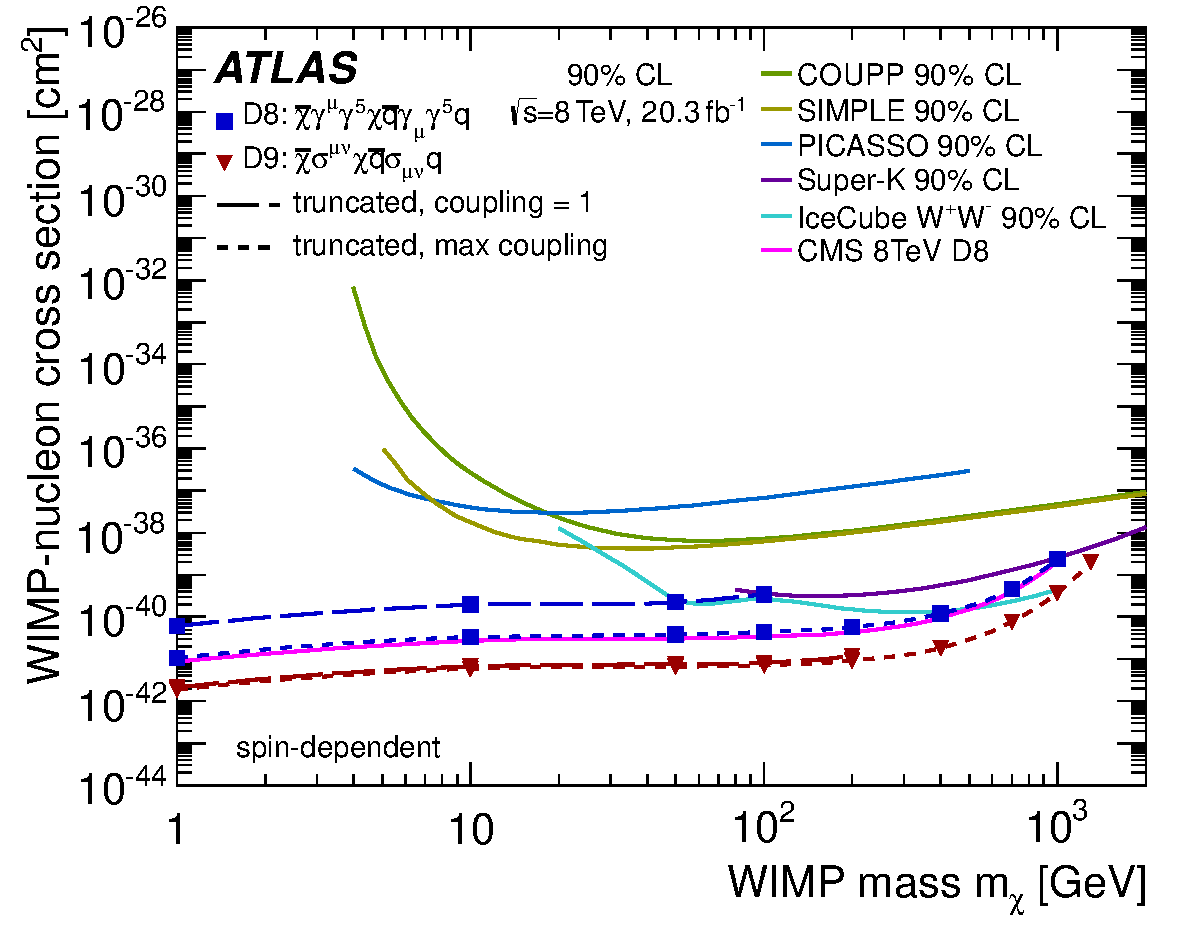
\includegraphics[width=0.35\textwidth]{figures/Monojet8TeV_EFT_SD}
%Can't have both so choose less controversial
%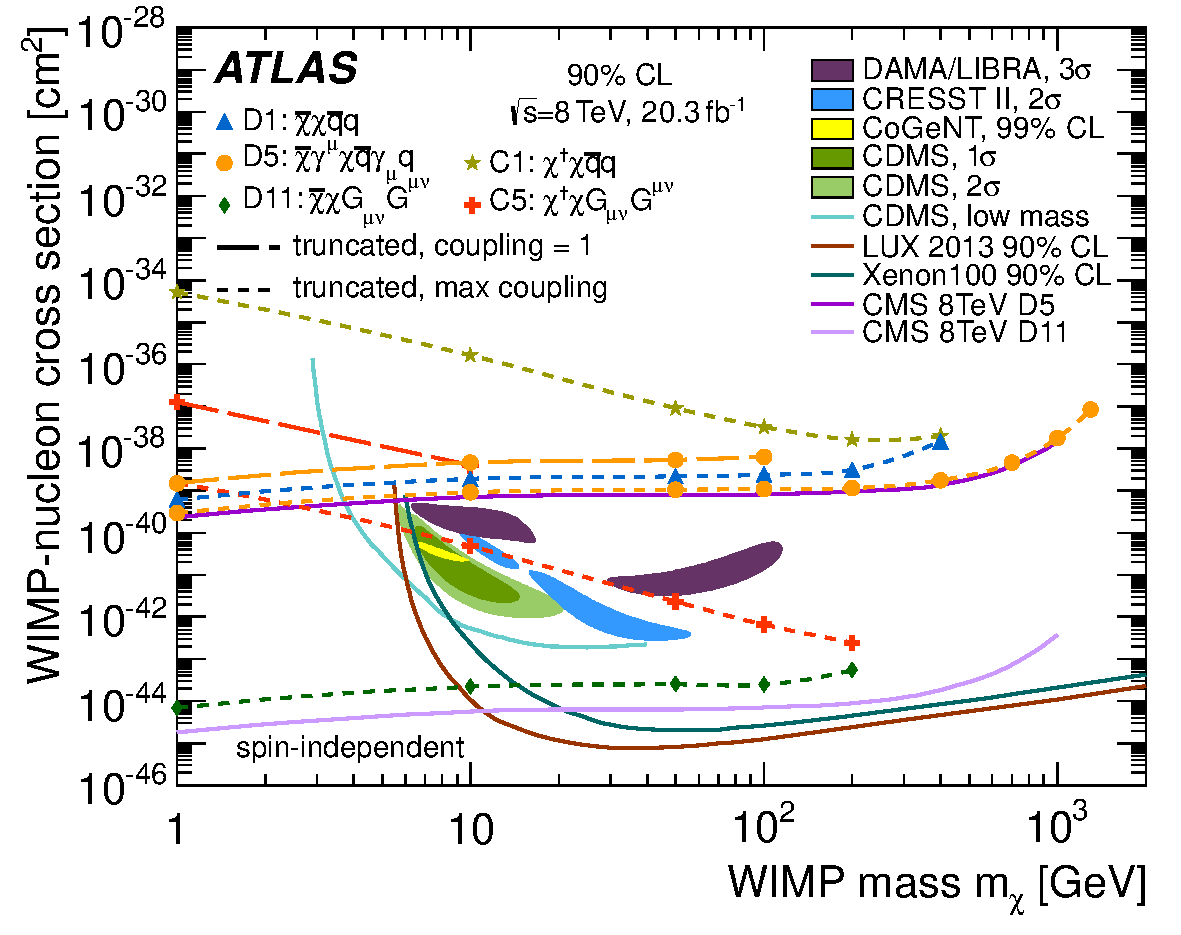
\includegraphics[width=0.9\textwidth]{figures/Monojet8TeV_EFT_SI}
%\caption{Inferred 90\% CL limits on (left) the spin-independent and (right) spin-dependent WIMP--nucleon scattering cross section as a function of DM mass m? for different operators. Results from direct-detection experiments for the spin-independent and spin-dependent cross section, and the CMS (untruncated) results are shown for comparison. From~\cite{monoXfig}.}
%\label{fig:SIATLASEFT}
%\end{figure}


%Mention Gambit? I would rather describe it in the "SUSY fits" part

%We aren't talking about uncertainties on DD and ID, maybe we should or at least we should cite?
%https://arxiv.org/abs/1409.5446


%\subsection{Comparing LHC constraints from visible and invisible searches with the DM relic density}



%Confronting the entire set of collider results with the relic density using a full model requires a 
%careful framework that is able to test model points against data. A variety of tools are available for this purpose,
%notably Mastercode~/cite{MC} and Gambit~/cite{G}. [Do we want to describe? Sentence is empty this way but we have no more space]. 

%DMWG 
%Relic density calculations can be overlaid on the mass-mass plot to indicate where the particles and interactions of a specific simplified model are by themselves su cient for explaining the observed DM abundance. For the simplified models recommended by the ATLAS/CMS DM Forum, this curve corresponds to the parameters for which the observed relic abundance is compatible with a single species of DM Dirac fermion and a single mediator that couples to all SM quarks with equal strength. One should not conclude that a simplified model is ruled out for values of model parameters that are inconsistent with the relic density overlay. Rather, one should conclude that additional physics beyond the simplified model was relevant for determining the DM abundance in the early Universe.



%%%%%THIS IS ALL STUFF FROM CHAPTER 3

\subsection{Stuff from chapter 3}

\subsubsection{monoZ}
%MonoZ


The LEP precision measurements~\footnote{Bounds on Z to invisible decays obtained from LHC searches are not yet competitive~\cite{deSimone:2014pda}.}, as well as direct detection experiments, rule out the majority of the Z-mediated invisible particles scenarios~\cite{Arcadi:2014lta,Escudero:2016gzx}. The LEP invisible width is well below the width one would expect if vector and axial vector models of invisible particles were realized, for all couplings satisfying the relic density with a invisible particles mass below 25 GeV. Direct detection experiments such as Xenon1T~\cite{Aprile:2017iyp} 
%CD: take figure 2 of Escudero:2016gzx and compare with the results of Aprile:2017iyp
rule out most of the other simplified model scenarios compatible with freeze-out relic density up to multi-TeV invisible particles masses. 
%invisible particles mass above 6 TeV for the vector couplings, while for axial the plot is truncated. 

%%Text from before

The invisible decays of the Z and Higgs boson are the main direct targets of searches for SM-boson-mediated interactions between SM and invisible particles particles, if the invisible particles particle is lighter than half the mass of the boson. Above this region, Direct Detection experiments are generally more sensitive than collider experiments. 


If the invisible particles mass is below half the mass of the Z, the Z can decay into invisible particles leading to strong constraints by LEP. Direct detection experiments constrain the rest of the parameter space 
where the relic density is satisfied. 
constrained by LEP and direct detection experiments (see e.g. Refs.~\cite{Arcadi:2014lta,Escudero:2016gzx}).

In $SU(2)_L \times U(1)$ extensions of the SM, the axial and vector couplings of the Z boson to invisible particles are generally required to be of the same order. If no other couplings are present, this model is not $SU(2) \times U(1)$ invariant, unless couplings to the invisible particles to the Higgs boson are added as well~\cite{Kahlhoefer:2015bea}. 
%The couplings between the Z and the invisible particles can be vector, axial or mixed. 
In the minimal case where the couplings do not depend on the Lorentz structure of the interaction, 
%what I want to say: In general they are excluded in their minimal version because of their strong vectorial coupling necessary to respect relic abundance bounds.
large couplings are required for this model to satisfy the relic density. 
In the case of equal vector and axial couplings, this model is heavily 

This model can still be viable wherever no relations between the vector and axial couplings are present. A review of Z portal models with different couplings can be found in Ref.~\cite{Arcadi:2014lta}. 
%Does one require a certain kind of couplings for symmetries? 
%Arcadi says: 
%In all these extensions, the axial coupling Aχ (see eq.(1)) of the Z boson to the invisible particles is naturally of the order of magnitude of its vectorial coupling Vχ. The deep reason is that in a framework of SU(2)L × U(1) breaking the original SU(2)L condition (Vχ = Aχ) is only mildly modified by the dynamic of the breaking. 
%Maybe link this to the choices for the Z' model later on? 

%%End text from before

\subsubsection{H portal}

%What does it mean for Higgs portal models: DD is always better
In the case of light fermion invisible particles with scalar couplings to the Higgs, direct detection experiment rule out most of the parameter space where the model can provide the measured relic density~\cite{Escudero:2016gzx,Djouadi:2011aa}. Due to the suppression of the cross-section for DD in the pseudoscalar case, the model is still not constrained around a small region for invisible particles masses corresponding to half the Higgs mass and above. %CD: maybe we have to say why this is the case - essentially rates are too small, see paper by Plehn. 

\subsubsection{Monojet}

%V/AV come from CMS search, ATLAS is less sensitive as it's 1.55 TeV
Vector and axial vector mediators are excluded by LHC searches at values of \mdm particles up to 700 and 400 GeV respectively with \mmed up to 1.8 TeV. This choice of model and couplings produces a relic density that is lower than the Planck measurement and it is still unconstrained by LHC searches for \mdm particles$>$0.3 TeV at \mdm particles$=$1.8 TeV for the vector mediator, and for 0.65$<$\mdm particles$<$0.75 TeV at \mdm particles=1.8 TeV for the axial vector mediator\footnote{Here and in the following, we quote observed limits at 95\% C.L. and refer to the bibliography for expected limits and 90\% C.L. limits.}. 
